\documentclass[russian,14pt,twoside]{extreport}
\usepackage[T2A]{fontenc}
\usepackage[utf8]{inputenc}
\usepackage[russian]{babel}
%%----------------------------------------------------------------------------
\usepackage{setspace}
\selectfont
\parindent=18pt
\frenchspacing
%%----------------------------------------------------------------------------
\usepackage{amsmath}
\usepackage{amssymb}
\usepackage{amscd}
\usepackage{amsthm}
\usepackage{etoolbox}
%\usepackage{mathtools}
\usepackage{bm}
\usepackage{titlesec}
\usepackage{caption}
\usepackage{graphicx}
\usepackage{listings}
\usepackage[all]{xy}
\usepackage{url}
\usepackage{array}
\usepackage{tabularx}
\usepackage{booktabs}
%%----------------------------------------------------------------------------
\usepackage[%
        a4paper,%
        includehead,%
        left=2cm,%
        top=2cm,%
        right=2cm,%
        bottom=2cm,%
        headheight=0.7cm,%
        headsep=0.3cm,%
        footskip=1.6cm]{geometry}
\special{papersize=210mm,297mm}
%%----------------------------------------------------------------------------
\renewcommand{\thefootnote}{\fnsymbol{footnote}}
%%----------------------------------------------------------------------------
\usepackage{fancyhdr}
\pagestyle{fancy}%
\fancyhead{}%
\fancyfoot{}%
\fancyhead[LE,RO]{\normalsize \thepage}%
\fancyhead[RE,LO]{\leftmark}
%%----------------------------------------------------------------------------
\raggedbottom
%%----------------------------------------------------------------------------
\makeatletter
%%----------------------------------------------------------------------------
\protected\def\switchinitials#1{%
\begingroup%
\edef\temp{\endgroup%
    \noexpand\switchinitials@fixcomma%
    \forcsvlist{\switchinitials@item}{#1}\relax}%
    \temp}
\def\switchinitials@fixcomma, #1{#1}
\def\switchinitials@item#1{, \switchinitials@single#1\relax}
\def\switchinitials@single#1~#2\relax{#2~#1}
%% Счетчик для списка авторов в колонтитуле
\newcounter{headauthorscounter}
\def\saveauthor#1{%
    \stepcounter{headauthorscounter}%
    \expandafter\def\csname headauthorslist\theheadauthorscounter%
        \endcsname{#1}}
\def\ifnthauthor#1{%
    \ifcsname headauthorslist#1\endcsname}
\def\getnthauthor#1{%
    , \csname headauthorslist#1\endcsname}
\def\putnthauthor#1{%
    \ifnthauthor#1\getnthauthor#1\fi}
\def\getfirstivauthors{%
    \noexpand\switchinitials@fixcomma%
    \putnthauthor1\putnthauthor2\putnthauthor3\putnthauthor4%
    \ifnthauthor5 и др.\fi}
%%----------------------------------------------------------------------------
\newenvironment{lmrarticle}[3][russian]{%
\setcounter{figure}{0}
\setcounter{equation}{0}
\setcounter{definition}{0}
\setcounter{theorem}{0}
\setcounter{lemma}{0}
\setcounter{statement}{0}
\setcounter{remark}{0}
\setcounter{corollary}{0}
\pagebreak[2]
\vskip 12pt plus 6pt minus 3pt
\vglue 4pt plus 2pt minus 2pt
{\leftskip=1.5\parindent
\rightskip=1.5\parindent
\vbox{\centering\sffamily\scshape\bfseries\boldmath\Large #2\unboldmath}}
\setcounter{headauthorscounter}{0}
\forcsvlist{\saveauthor}{#3}
\markboth{\getfirstivauthors}{}
\nopagebreak
\vskip 6pt
\@afterheading
}{%
}
%%----------------------------------------------------------------------------
\newcommand\OneAuthor[3]{%
\vbox{%
{\centering\bfseries\normalsize #1\par}
\vskip 3pt
\raggedright
\leavevmode\noindent\footnotesize
\hangindent=18pt\hangafter=1
#2, e-mail: \texttt{#3}\\*\par}
\nopagebreak
\medskip
\@afterheading
}
%%----------------------------------------------------------------------------
\newcommand\TwoAuthor[6]{%
\vbox{%
{\centering\bfseries\normalsize #1$^1$, #4$^2$\\}
\vskip 3pt
\raggedright
\leavevmode\noindent\footnotesize
\hangindent=18pt\hangafter=1
$^1$ {#2}, e-mail: \texttt{#3}\par
\hangindent=18pt\hangafter=1
$^2$ {#5}, e-mail: \texttt{#6}\\*\par}
\nopagebreak
\smallskip
\@afterheading
}
%%----------------------------------------------------------------------------
\newcommand\ThreeAuthor[9]{%
\vbox{%
{\centering\bfseries\normalsize #1$^1$, #4$^2$, #7$^3$\\}
\vskip 3pt
\raggedright
\leavevmode\noindent\footnotesize
\hangindent=18pt\hangafter=1
$^1$ {#2}, e-mail: \texttt{#3}\par
\hangindent=18pt\hangafter=1
$^2$ {#5}, e-mail: \texttt{#6}\par
\hangindent=18pt\hangafter=1
$^3$ {#8}, e-mail: \texttt{#9}\\*\par}
\nopagebreak
\smallskip
\@afterheading
}
%%----------------------------------------------------------------------------
\newcommand\FourAuthor[9]{%
\def\Argi{{#1}}%
\def\Argii{{#2}}%
\def\Argiii{{#3}}%
\def\Argiv{{#4}}%
\def\Argv{{#5}}%
\def\Argvi{{#6}}%
\def\Argvii{{#7}}%
\def\Argviii{{#8}}%
\def\Argix{{#9}}%
\FourAuthorContinue
}
\newcommand\FourAuthorContinue[3]{%
\vbox{%
{\centering
{\bfseries\normalsize \Argi$^1$, \Argiv$^2$, \Argvii$^3$, #1$^4$\\}}
\vskip 3pt
\raggedright
\leavevmode\noindent\footnotesize
\hangindent=18pt\hangafter=1
$^1$ \Argii, e-mail: \texttt{\Argiii}\par
\hangindent=18pt\hangafter=1
$^2$ \Argv, e-mail: \texttt{\Argvi}\par
\hangindent=18pt\hangafter=1
$^3$ \Argviii, e-mail: \texttt{\Argix}\par
\hangindent=18pt\hangafter=1
$^4$ #2, e-mail: \texttt{#3}\\*\par}
\nopagebreak
\smallskip
\@afterheading
}
%%----------------------------------------------------------------------------
\newcommand\FiveAuthor[9]{%
\def\Argi{{#1}}%
\def\Argii{{#2}}%
\def\Argiii{{#3}}%
\def\Argiv{{#4}}%
\def\Argv{{#5}}%
\def\Argvi{{#6}}%
\def\Argvii{{#7}}%
\def\Argviii{{#8}}%
\def\Argix{{#9}}%
\FiveAuthorContinue
}
\newcommand\FiveAuthorContinue[6]{%
\vbox{%
{\centering
\bfseries\normalsize \Argi$^1$, \Argiv$^2$, \Argvii$^3$, #1$^4$, #4$^5$\\}
\vskip 3pt
\raggedright
\leavevmode\noindent\footnotesize
\hangindent=18pt\hangafter=1
$^1$ {\Argii}, e-mail: \texttt{\Argiii}\par
\hangindent=18pt\hangafter=1
$^2$ {\Argv}, e-mail: \texttt{\Argvi}\par
\hangindent=18pt\hangafter=1
$^3$ {\Argviii}, e-mail: \texttt{\Argix}\par
\hangindent=18pt\hangafter=1
$^4$ {#2}, e-mail: \texttt{#3}\par
\hangindent=18pt\hangafter=1
$^5$ {#5}, e-mail: \texttt{#6}\\*\par}
\nopagebreak
\smallskip
\@afterheading
}
%%----------------------------------------------------------------------------
\titleformat{\paragraph}[runin]{\bfseries}{}{0pt}{}
\titleformat{\section}{\bfseries}{}{0pt}{}
\let\subsection\@undefined
\let\subsubsection\@undefined
\let\subparagraph\@undefined
%%----------------------------------------------------------------------------
\newtheorem{definition}{\protect\definitionname}
\newtheorem*{definition*}{\protect\definitionname}
\newtheorem{theorem}{\protect\theoremname}
\newtheorem*{theorem*}{\protect\theoremname}
\newtheorem{lemma}{\protect\lemmaname}
\newtheorem*{lemma*}{\protect\lemmaname}
\newtheorem{statement}{\protect\statementname}
\newtheorem*{statement*}{\protect\statementname}
\newtheorem{remark}{\protect\remarkname}
\newtheorem*{remark*}{\protect\remarkname}
\newtheorem{corollary}{\protect\corollaryname}
\newtheorem*{corollary*}{\protect\corollaryname}
\newcommand{\definitionname}{}
\newcommand{\theoremname}{}
\newcommand{\lemmaname}{}
\newcommand{\statementname}{}
\newcommand{\remarkname}{}
\newcommand{\corollaryname}{}
\addto\captionsrussian{%
  \renewcommand{\definitionname}{Определение}%
  \renewcommand{\theoremname}{Теорема}%
  \renewcommand{\lemmaname}{Лемма}%
  \renewcommand{\statementname}{Утверждение}%
  \renewcommand{\remarkname}{Замечание}%
  \renewcommand{\corollaryname}{Следствие}%
}
%%----------------------------------------------------------------------------
\usepackage{enumitem}
\setlist[enumerate]{%
    %labelindent=0pt by default
    leftmargin=*,%
    topsep=4pt plus 2pt minus 2pt,%
    partopsep=2pt plus 1pt minus 1pt,%
    parsep=2pt plus 1pt,%
    itemsep=2pt plus 1pt%
}
\setlist[itemize]{%
    %labelindent=0pt by default
    label={---},%
    leftmargin=*,%
    topsep=4pt plus 2pt minus 2pt,%
    partopsep=2pt plus 1pt minus 1pt,%
    parsep=2pt plus 1pt,%
    itemsep=2pt plus 1pt%
}
%%----------------------------------------------------------------------------
\newenvironment{lmrreferences}{
\pagebreak[1]
\medskip
\noindent
{\scshape\large Список литературы}
\par\nopagebreak
\smallskip
\@afterheading
\begin{enumerate}[label={[\arabic*]},leftmargin=*]
\sloppy
}{
\end{enumerate}
}
%%----------------------------------------------------------------------------
\binoppenalty=10000
\relpenalty=10000
\@clubpenalty=10000
\clubpenalty=10000
\widowpenalty=10000
%%----------------------------------------------------------------------------
%%----------------------------------------------------------------------------
\let\le\leqslant
\let\leq\leqslant
\let\ge\geqslant
\let\geq\geqslant
\let\emptyset\varnothing
\apptocmd\normalsize{%
  \abovedisplayskip=6pt plus 4pt minus 3pt
  \belowdisplayskip=6pt plus 4pt minus 3pt
  \abovedisplayshortskip=3pt plus 6pt minus 1pt
  \belowdisplayshortskip=3pt plus 6pt minus 1pt
}
%%----------------------------------------------------------------------------
\titlespacing*{\paragraph}{\parindent}{0pt}{4pt}
%%----------------------------------------------------------------------------
%%----------------------------------------------------------------------------
\makeatother
%%----------------------------------------------------------------------------
\begin{document}
\begin{lmrarticle}%
{О пяти свойствах булевых функций}{Образцов~О.\,О., Примеров~П.\,П.}
\TwoAuthor%
{Образцов Орест Орестович}%
    {Кафедра примеров и образцов}{obrazcov\_oo@emsu.ru}%
{Примеров Петр Петрович}%
    {Кафедра шаблонов и трафаретов}{primerov\_pp@cs.msu.ru}

% Другие примеры:
%
% \OneAuthor%
% {Образцов Орест Орестович}%
%   {Эмский университет}{obrazcov\_oo@emsu.ru}%
%
% \ThreeAuthor%
% {Образцов Орест Орестович}%
%    {Кафедра примеров и образцов}{obrazcov\_oo@emsu.ru}%
% {Примеров Петр Петрович, Трафаретов Тимофей Тимофеевич}%
%    {Юмский университет}{primerov\_pp@yumsu.ru, trafaretov\_tt@yumsu.ru}

Это "--- пример оформления файла статьи. Сами правила оформления содержатся в
файле \texttt{lmr21\_guide.pdf}. Пример ссылок на статьи~[1,\,2,\,3],
диссертацию~[4], книгу~[5]. Обратите внимание на оформление ссылки~[3] на
статью с четырьмя и более авторами. Ссылки на статьи ставятся вручную.
\begin{figure}[ht]
\centering
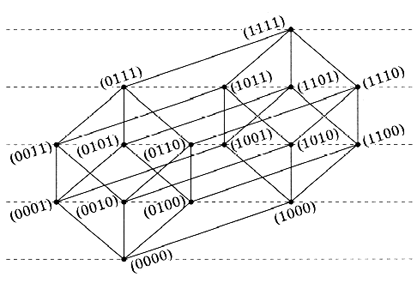
\includegraphics[width=0.6\textwidth]{bcube}
\caption{Слои булевого куба.}
\label{fi:bcube}
\end{figure}

% Раздел можно задать командой \paragraph{Название раздела}
\paragraph{Название раздела.}
Предусмотрено применение команд как использующих глобальную систему
нумерации, так и вариантов этих команд со звёздочкой, которые её не используют.
Например, ссылка на рисунок~\ref{fi:bcube} сгенерирована автоматически, а на
рисунок~2 "--- проставлена вручную, при этом в первом случае для задания
подписи к рисунку используется команда \verb|\caption|, а во втором "---
команда
\verb|\caption*|.
\begin{figure*}[ht]
\centering
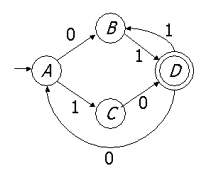
\includegraphics[width=5cm]{smach}
\caption*{Рис.~2: Пример инициального автомата.}
\end{figure*}

% Для вёрстки абзацев с переполнением строк можно
% воспользоваться окружением sloppypar
\begin{sloppypar}
Для создания выключных формул надо пользоваться окружениями \texttt
{equation}, \texttt {gather}, \texttt {multline} и др. подобными им, а также их
вариантами со звёздочкой, которые не проставляют номер формулы. При этом не
следует задавать выключные формулы с использованием команды \verb|$$|,
в~крайнем случае для этого можно воспользоваться командами \verb|\[|, \verb|\]|
(не рекомендуется). Например:
\end{sloppypar}
\begin{equation}
\label{eq:stdbase}
[\{x \&y, x \vee y, {\bar x}\}] = P_2.
\end{equation}
Для нумерации формул вручную можно воспользоваться окружением со звёздочкой и
командой~\verb|\eqno|, при этом ссылка~(2) на такую формулу также проставляется
вручную:
\begin{equation*}
\label{eq:polbase}
[\{x \oplus y, x \& y, 1, 0 \}] = P_2. \eqno{(2)}
\end{equation*}
Тезисы не должны содержать нумерованых формул, на которые нет ссылок в тексте.

% Иногда требуется, чтобы TeX сверстал параграф на одну строку короче.
% Пример показывает как этого добиться указанием команды \looseness=-1
% перед завершением следующего параграфа.
В~тексте предусмотрено использование предопределённых окружений типа
\texttt{theorem} пакета \texttt{amsthm}. Для определений, лемм, утверждений,
теорем, замечаний, следствий предлагается использовать окружения следующего
вида:\looseness=-1
\begin{definition*}
Базис $\{x \& y, x \vee y, {\bar x}\}$ называется \emph{стандартным}.
\end{definition*}
\begin{lemma}
\label{lm:nonullfn}
Формулировка леммы о ненулевой функции.
\end{lemma}
\begin{proof}
\begin{sloppy}
Доказательство леммы~\ref{lm:nonullfn}, использующее формулу~\eqref{eq:stdbase}
и заканчивающееся выключной формулой (обратите внимание на команду
\verb|\qedhere| в этом случае):
\begin{equation*}
f \neq 0. \qedhere%
\end{equation*}
\end{sloppy}
\end{proof}
\begin{statement}
\label{st:canonrep}
Формулировка устверждения о каноническом разложении функции.
\end{statement}
\begin{remark*}
Заметим, что в утверждении~\ref{st:canonrep} канонический вид единственный с
точностью до перестановки слагаемых.
\end{remark*}
\begin{theorem}
\label{th:fivebf}
Формулировка теоремы о пяти булевых функциях.
\end{theorem}
\begin{proof}
Текст доказательства теоремы~\ref{th:fivebf}.
\end{proof}
\begin{corollary*}
Формулировка следствия из теоремы~\ref{th:fivebf}.
\end{corollary*}
Все перечисленные выше окружения можно использовать как в вариантах со
звёздочкой, так и без.

Авторы выражают благодарность профессору Шаблонову~С.\,С. за постановку задачи.

Работа выполнена при поддержке РФФИ (проект \hbox{№\,15-01-12345-а}).

% Библиография создается вручную при помощи окружения lmrreferences,
% которое является разновидностью окружения enumerate
\begin{lmrreferences}
\item
Образцов~О.\,О. Некоторые свойства булевых функций~// Труды XXIV
Международной конференции <<Достижения отечественной микроэлектроники>>
(Эмск, 21--27 июня 2197\,г.). Э.~: ЗАРЯ Пресс, 2197. С.\,502--507.
\item
Образцов~О.\,О., Примеров~П.\,П., Шаблонов~Ш.\,Ш. О~свойствах
$k$"=значных функций~// Вестник Эмского государственного университета. Серия 9.
Математическая кибернетика. 2015. Т.\,1, №\,2. С.\,33--47.
\item
Некоторые свойства автоматных функций~/ О.\,О.~Образцов, П.\,П.~Примеров,
Ш.\,Ш.~Шаблонов, Т.\,Т.~Трафаретов~// Вестник Юмского государственного
университета. Серия 7.  Дискретная математика. 2016. Т.\,3, №\,1.  С.\,10--25.
\item
Примеров~П.\,П. Методы оценки сложности недоопределенных булевых
функций~: дис.  \ldots\ канд. физ.-мат. наук~: 01.01.09~/ Примеров Петр
Петрович. Юмск, 2013. 199\,с.
\item
Львовский~С.\,М. Набор и вёрстка в системе \LaTeX. М.~: МЦНМО,
2006. 448\,с.
\end{lmrreferences}
\end{lmrarticle}

\end{document}
